% IEEE standard conference template; to be used with:
%   spconf.sty  - LaTeX style file, and
%   IEEEbib.bst - IEEE bibliography style file.
% --------------------------------------------------------------------------

\documentclass[letterpaper]{article}
\usepackage[T1]{fontenc}
\usepackage[utf8]{inputenc}
\usepackage{spconf,amsmath,amssymb,graphicx}
\usepackage[colorinlistoftodos]{todonotes}

\newcommand{\mytodo}[1]{\todo[inline]{#1}}
\newcommand{\dtodo}[1]{\todo[inline, color=cyan]{#1}}
\newcommand{\rtodo}[1]{\todo[inline, color=yellow]{#1}}
\newcommand{\ptodo}[1]{\todo[inline, nolist, color=green]{#1}}

% Example definitions.
% --------------------
% nice symbols for real and complex numbers
\newcommand{\R}[0]{\mathbb{R}}
\newcommand{\C}[0]{\mathbb{C}}

% bold paragraph titles
\newcommand{\mypar}[1]{{\bf #1.}}

% Title.
% ------
\title{Optimizing Simplex Implementation For Standard Form Problems}
%
% Single address.
% ---------------
\name{Donjan Rodic, Rico Häuselmann} 
\address{Department of Mathematics\\ ETH Zürich\\Zürich, Switzerland}

% For example:
% ------------
%\address{School\\
%		 Department\\
%		 Address}
%
% Two addresses (uncomment and modify for two-address case).
% ----------------------------------------------------------
%\twoauthors
%  {A. Author-one, B. Author-two\sthanks{Thanks to XYZ agency for funding.}}
%		 {School A-B\\
%		 Department A-B\\
%		 Address A-B}
%  {C. Author-three, D. Author-four\sthanks{The fourth author performed the work
%		 while at ...}}
%		 {School C-D\\
%		 Department C-D\\
%		 Address C-D}
%

\begin{document}
%\ninept
%
\maketitle
%

\listoftodos

\begin{abstract}
\ptodo{Describe in concise words what you do, why you do it (not necessarily
in this order), and the main result.  The abstract has to be
self-contained and readable for a person in the general area. You
should write the abstract last.}
\end{abstract}

\section{Introduction}\label{sec:intro}

In this section we will motivate our choice of algorithm to optimize and give
a brief overview of related work.

\mypar{Motivation} The Simplex algorithm for linear optimization is widely
used \mytodo{add examples}

Performance can be very critical in some applications when 
optimizing a linear problem is a crucial part of decision making.
\mytodo{add reasons and examples}

\mypar{Implementation} We present an implementation which is optimized 
for a limited class of linear optimization problems and solves this kind of problem
faster than any commerciably available general purpose solver.

\mypar{Related work} \mytodo{cite original danzig paper, handouts from opti, papers of the other implementations.}

\section{Background: The Simplex Algorithm}\label{sec:background}

\mypar{Linear Optimization Problems} \mytodo{put the Max c'x Subject to \dots formula and explain}

\mypar{Standard form Problems} \mytodo{explain standard form, mention restriction to standard form}
% standard form restrictions result from trying to keep the focus more on optimization and less on implementing a domain specific language parser.

\mypar{The Simplex Method} \mytodo{explain Simplex in tableau form}

\mypar{Cost Analysis}
\mytodo{mention number of iterations varies with problem matrix}

\mytodo{cost analysis for one iteration}

\section{Your Proposed Method}\label{sec:yourmethod}

In this section we explain the our baseline implementation as well as all optimizations we made.
\ptodo{Now comes the ``beef'' of the paper, where you explain what you
did. Again, organize it in paragraphs with titles. As in every section
you start with a very brief overview of the section.}

\ptodo{For this class, explain all the optimizations you performed. This mean, you first very briefly
explain the baseline implementation, then go through locality and other optimizations, and finally SSE (every project will be slightly different of course). Show or mention relevant analysis or assumptions. A few examples: 1) Profiling may lead you to optimize one part first; 2) bandwidth plus data transfer analysis may show that it is memory bound; 3) it may be too hard to implement the algorithm in full generality: make assumptions and state them (e.g., we assume $n$ is divisible by 4; or, we consider only one type of input image); 4) explain how certain data accesses have poor locality. Generally, any type of analysis adds value to your work.}

\mytodo{
\mypar{Baseline Implementation}
}
Our baseline implementation parses an input file containing the coefficients for the objective function and the constraints.
The coefficients are stored in a two dimensional STL vector of vector representation of the simplex tableau.

The steps performed in each iteration are separated into three functions: 
\begin{itemize}
    \item{\tt pivot\_col}
    \item{\tt pivot\_row}
    \item{\tt base\_exchange}
\end{itemize}
The first two contain the code for finding the pivot element to use in the iteration whereas
the third facilitates the gaussian elimination step.

Profiling was done with gprof, perf and valgrind. All tools consistently showed that the vast majority of the
runtime is spent in the {\tt base\_exchange} function, where we focused all subsequent optimization.
Further annotated analysis revealed stalls at the memory access functions, which can be alleviated via ILP via static scalar assignment
where unit stride access was applicable.


\rtodo{
\mypar{Array}
}
The Array optimization replaces the vector of vectors implementation of the tableau by
a C99 one dimensional contiguous array allocated and aligned using {\tt \_mm\_alloc } from
the intel intrinsics headers.

All subsequent optimizations were based on this implementation.

\dtodo{
\mypar{Cache control}
}
Cache control was attempted through intrinsics for nontemporal assignment in order to avoid polluting the cache with updates on the active basis elements and
effective cost calculations. We further added prefetching in order to load soon-to-be-used blocks into the L2 cache.

\rtodo{
\mypar{Blocking}
}
As a next step we did blocking in the loop that runs over the whole tableau 
inside the basis exchange

\mytodo{
\mypar{Vectorization}
}

\ptodo{As important as the final results is to show that you took a structured, organized approach to the optimization and that you explain why you did what you did.}

\ptodo{Mention and cite any external resources including library or other code.}

\ptodo{Good visuals or even brief code snippets to illustrate what you did are good. Pasting large amounts of code to fill the space is not good.}

\section{Experimental Results}\label{sec:exp}

\ptodo{Here you evaluate your work using experiments. You start again with a
very short summary of the section. The typical structure follows.}

\mypar{Experimental setup} \ptodo{Specify the platform (processor, frequency, cache sizes)
as well as the compiler, version, and flags used. I strongly recommend that you play with optimization flags and consider also icc for additional potential speedup.}

\ptodo{Then explain what input you used and what range of sizes. The idea is to give enough information so the experiments are reproducible by somebody else on his or her code.}
\mytodo{mention problem generator, instrumentalization, use of third party code.}

\mypar{Results}

Profiling of the {\tt swapNxM\_block } implementations showed that between 70\% and 90\% of the time is spent on\\
{\tt \_mm256\_load\_pd } calls.

As shown in Fig.~\ref{res_cachecontrol}, nontemporal assignment showed a negligible effect on the swapping implementations,
while prefetching lead to a considerable slowdown.


\begin{figure}\centering
  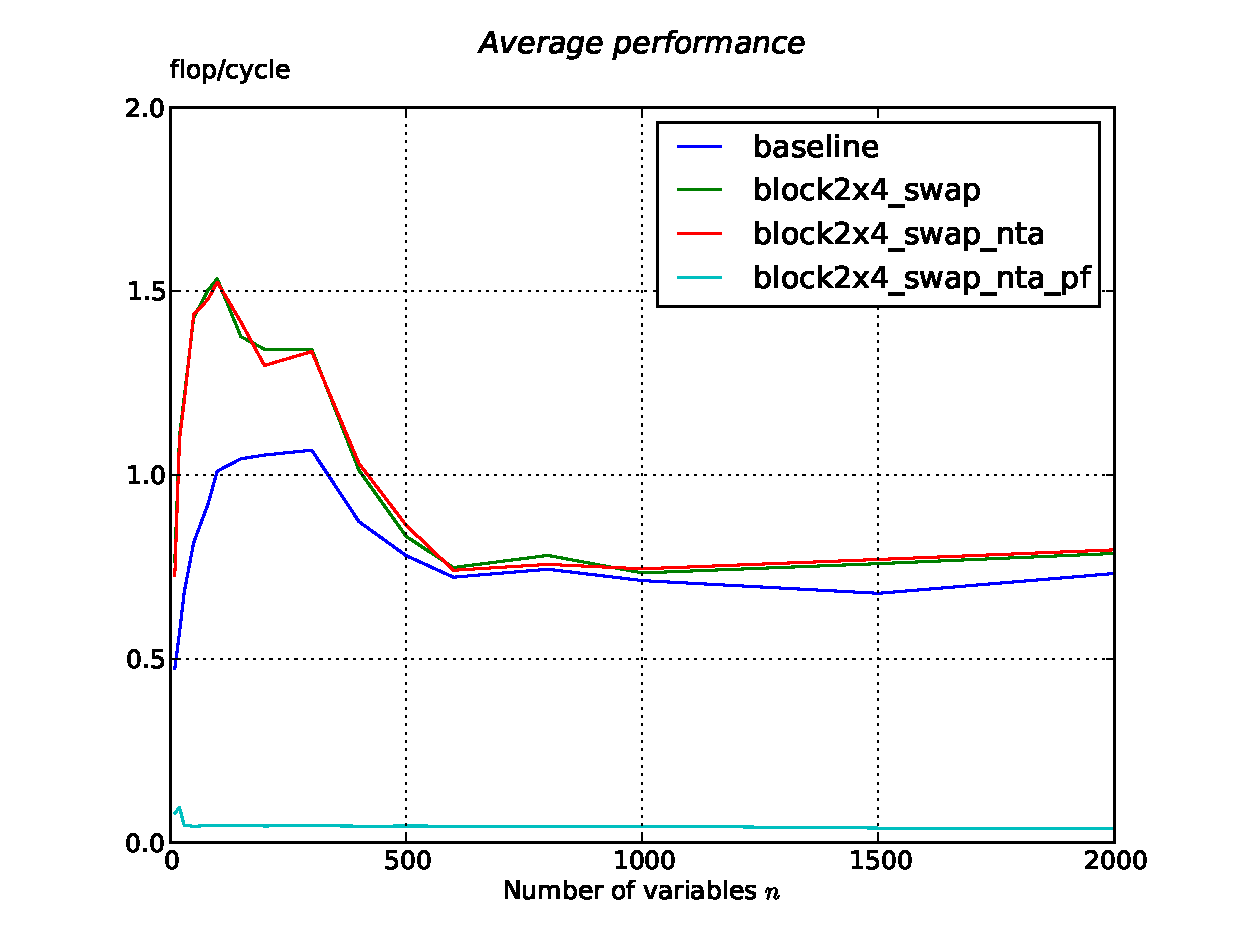
\includegraphics[scale=0.4]{img/results_cachecontrol.eps}
  \caption{Performance of nontemporal assignment ({\tt \_nta}) and prefetching ({\tt \_nta\_pf}) implementations of {\tt block2x4\_swap} and the baseline,
  all with the same operation count.\label{res_cachecontrol}}
\end{figure}

\ptodo{Next divide the experiments into classes, one paragraph for each. In the simplest case you have one plot that has the size on the x-axis and the performance on the y-axis. The plot will contain several lines, one for each relevant code version. Discuss the plot and extract the overall performance gain from baseline to best code. Also state the percentage of peak performance for the best code. Note that the peak may change depending on the situation. For example, if you only do additions it would be 12 Gflop/s
on one core with 3 Ghz and SSE and single precision floating point.

Do not put two performance lines into the same plot if the operations count changed significantly (that's apples and oranges). In that case first perform the optimizations that reduce op count and report the runtime gain in a plot. Then continue to optimize the best version and show performance plots.}

\ptodo{{\bf You should}
\begin{itemize}
\item Follow the guide to benchmarking presented in class, in particular
\item very readable, attractive plots (do 1 column, not 2 column plots
for this class), proper readable font size. An example is below (of course you can have a different style),
\item every plot answers a question, which you pose and extract the
answer from the plot in its discussion
\end{itemize}
Every plot should be discussed (what does it show, which statements do
you extract).}

\section{Conclusions}

\ptodo{Here you need to briefly summarize what you did and why this is
important. {\em Do not take the abstract} and put it in the past
tense. Remember, now the reader has (hopefully) read the paper, so it
is a very different situation from the abstract. Try to highlight
important results and say the things you really want to get across
(e.g., the results show that we are within 2x of the optimal performance ... 
Even though we only considered the DFT, our optimization
techniques should be also applicable ....) You can also formulate next
steps if you want. Be brief.}

\section{Further comments}

\ptodo{Here we provide some further tips.

\mypar{Further general guidelines}

\begin{itemize}
\item For short papers, to save space, I use paragraph titles instead of
subsections, as shown in the introduction.

\item It is generally a good idea to break sections into such smaller
units for readability and since it helps you to (visually) structure the story.

\item The above section titles should be adapted to more precisely
reflect what you do.

\item Each section should be started with a very
short summary of what the reader can expect in this section. Nothing
more awkward as when the story starts and one does not know what the
direction is or the goal.

\item Make sure you define every acronym you use, no matter how
convinced you are the reader knows it.

\item Always spell-check before you submit (to me in this case).

\item Be picky. When writing a paper you should always strive for very
high quality. Many people may read it and the quality makes a big difference.
In this class, the quality is part of the grade.

\item Books helping you to write better: \cite{Higham:98} and \cite{Strunk:00}.

\item Conversion to pdf (latex users only): 

dvips -o conference.ps -t letter -Ppdf -G0 conference.dvi

and then

ps2pdf conference.ps
\end{itemize}
}

\ptodo{
\mypar{Graphics} For plots that are not images {\em never} generate (even as intermediate step)
jpeg, gif, bmp, tif. Use eps, which means encapsulate postscript, os pdf. This way it is
scalable since it is a vector graphic description of your graph. E.g.,
from Matlab, you can export to eps or pdf.

Here is an example of how to get a plot into latex
(Fig.~\ref{fftperf}). Note that the text should not be any smaller than shown.
}

\begin{figure}\centering
  %\includegraphics[scale=0.33]{dft-performance.eps}
  \caption{Performance of four single precision implementations of the
  discrete Fourier transform. The operations count is roughly the
  same. {\em The labels in this plot are too small.}\label{fftperf}}
\end{figure}



% References should be produced using the bibtex program from suitable
% BiBTeX files (here: bibl_conf). The IEEEbib.bst bibliography
% style file from IEEE produces unsorted bibliography list.
% -------------------------------------------------------------------------
\bibliographystyle{IEEEbib}
\bibliography{bibl_conf}

\end{document}

